\section{Potentialfeld zur Bahngenerierung und Kollisionsvermeidung}
\label{sec:Potential}
In diesem Abschnitt wird beschrieben, wie das Potentialfeld aufgebaut ist, das zur Generierung des Geschwindigkeitsvektors genutzt wird.
\subsection{Roboter Umwelt}
Um die statische Umwelt des Robotinos im Potentialfeld darzustellen, wird der zu befahrende Bereich in Zonen unterteilt. Die gew�hlten Zonen sind in Abbildung \ref{fig:PotZonen} farbig dargestellt. In Tabelle \ref{tab:Zonen} ist die Zuordnung der Zonen zur Abbildung \ref{fig:PotZonen} beschrieben. Dabei wird eine Hauptfahrzone (Zone 0) definiert, in der mit einem virtuellen Zaun der zu befahrene Bereich abgegrenzt wird. Dieser Zaun ist notwendig, damit die Zone nicht unkontrolliert verlassen wird, dazu werden e-Funktionen genutzt, die in den Funktionen \eqref{fun:H01} bis \eqref{fun:H03} definiert sind. Aufgrund der Form der Zone m�ssen dabei drei Funktionen definiert werden, die je nach Position des Robotinos ausgef�hrt werden. Das Verlassen der Zone 0 erfolgt durch die �bergabe an den Fertigungsbereich, welches in Kapitel \ref{sec:Kon_Bahnregelung} n�her erl�utert wird. \\
Zone 1 bis 3 dienen zur R�ckf�hrung der Robotinos zur Zone 0, dazu wird ein Potentialfeld genutzt, dass uns erm�glicht den Robotino in eine gezielte Richtung zu lenken. Die dazu genutzten Funktionen sind unter \eqref{fun:H1} bis \eqref{fun:H3} definiert. Diese Potentialfelder nutzen in Fahrrichtung eine Geradengleichung mit definierter Steigung und senkrecht dazu eine Parabelform, um den Robotino auf Kurs zu halten. Wenn sich der Robotino in Zone 4 befindet, wird dieser �ber eine Geradengleichung nach hinten gef�hrt. Die dabei genutzte Gleichung ist als \eqref{fun:H4} gekennzeichnet. Zus�tzlich wird in Zone 4 f�r jede Station eine gau�sche radiale Basisfunktion, welche unter Kapitel \ref{sec:PotRob} n�her erl�utert wird, genutzt, damit keine Kollision mit den Stationen auftreten. Diese Zone wird nur im Fehlerfall oder beim Start des Robotinos betreten, da in dieser Zone der Fertigungsbereich aktiv ist. Die Zone 5 dient dazu den Robotino gezielt in Richtung der Mitte der Zone 0 zu f�hren. Dazu wird, wie in Zone 1 bis 3, eine Parabel mit einer Geradengleichung genutzt. Die dabei genutzte Funktion ist als \eqref{fun:H5} definiert. Dabei ist zu beachten, dass vorgesehen ist, dass Zone 5 nur aktiv ist, wenn sie aus Zone 1 betreten wird. Dadurch wird die Anfahrm�glichkeit aus der Zone 0 zur Ladestation gew�hrleistet. \\
Je nach Zone gilt dabei ein eigenes Potentialfeld, welche kombiniert das Gesamtpotentialfeld ergebenen. Die einzelnen Zonen sind in Abbildung \ref{fig:Poteinzeln} dargestellt. Das gesamt Potentialfeld ist in Abbildung \ref{fig:PotUmweltohne} dargestellt, wobei zur �bersichtlichkeit die Stations und Ladestationspotentiale nicht dargestellt werden. Da die Zone 5 nur durchlaufen wird, wenn sie aus Zone 1 betreten wird, wird in Abbildung \ref{fig:PotUmweltmit} dargestellt, wie das Potentialfeld in diesem Fall aussieht.

\begin{table}
\centering
 \begin{tabular}{|c|c|c|}
  \hline Zone & Farbe & Beschreibung \\ 
  \hline 0 & ohne Farbe & Hauptfahrzone \\
  \hline 1 & Gr�n &  F�hrung des Robotinos nach Zone 5 \\
  \hline 2 & Blau &  F�hrung des Robotinos nach Zone 3 \\
  \hline 3 & Violet & F�hrung des Robotinos nach Zone 0 \\
  \hline 4 & Rot & F�hrung des Robotinos nach Zone 1 und 2\\
  \hline 5 & Cyan & F�hrung des Robotinos nach Zone 0 \\
   \hline \end{tabular}
   \caption{Zuordnung der Farben aus Abbildung \ref{fig:PotZonen}}
   \label{tab:Zonen}
\end{table}

\begin{figure}
	\centering	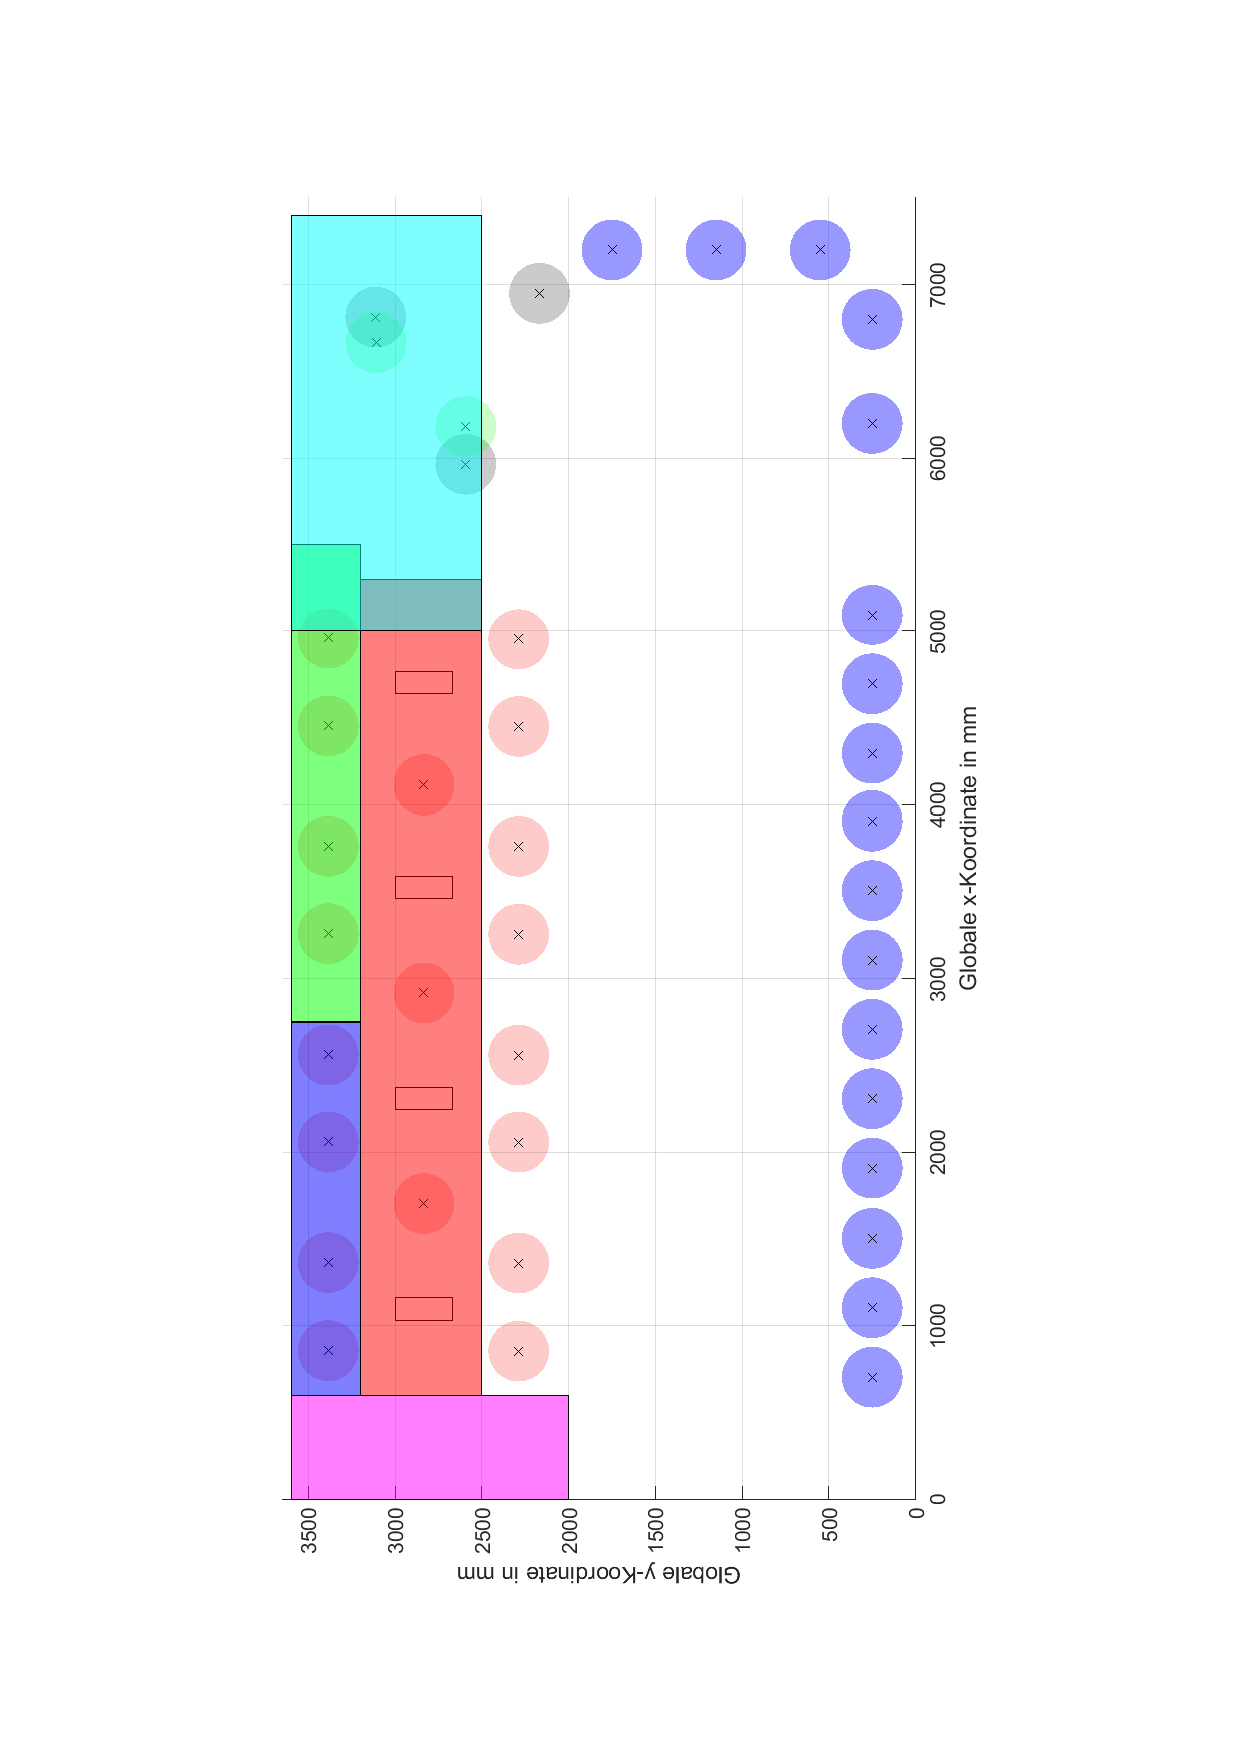
\includegraphics[width=0.8\textwidth, angle=-90]{grafiken/Zonen_eingezeichnet.pdf}
	\caption{Potentialfeldzonen}
	\label{fig:PotZonen}
\end{figure}

\scalebox{0.8}{\begin{minipage}{1.2\textwidth}
\begin{align}
\label{fun:H01}
H_{0(x=0..5500,y=0..2500)}(x,y)= K_{exp}\cdot(e^{(-\frac{x}{\sigma})}+e^{(\frac{x-7400}{\sigma})}+e^{(-\frac{y}{\sigma})}+e^{(\frac{y-2500}{\sigma})} ) \label{fun:H01}\\ 
\label{fun:H02}
H_{0(x=5500..7400,y=0..2500)}(x,y) = K_{exp}\cdot(e^{(-\frac{(x-5500)-(y-2500)}{\sigma})}+e^{(\frac{x-7400}{\sigma})}+e^{(-\frac{y}{\sigma})} )\\ 
\label{fun:H03}
H_{0(x=5500..7400,y=2500..3600)}(x,y) = K_{exp}\cdot(e^{(-\frac{(x-5500)}{\sigma})}+e^{(\frac{(y-3600)}{\sigma})}+e^{(\frac{x-7400}{\sigma})}+e^{(-\frac{y}{\sigma})} )\\ 
\label{fun:H1}
H_{1}(x,y) = - K_{gerade}\cdot x + K_{parabel}\cdot\frac{(y-3500)^2}{B}\\
\label{fun:H2}
H_{2}(x,y) = K_{gerade}\cdot x + K_{parabel}\cdot\frac{(y-3500)^2}{B}\\
\label{fun:H3}
H_{3}(x,y) = K_{parabel}\cdot\frac{(x-300)^2}{B} + K_{gerade}\cdot y\\
\label{fun:H4}
H_{4}(x,y) = - K_{gerade}\cdot y\\
\label{fun:H5}
H_{5}(x,y) = K_{parabel}\cdot\frac{(x-5500)^2}{B}-K_{gerade}\cdot y
 \end{align}
\end{minipage}

\begin{figure}
	\centering	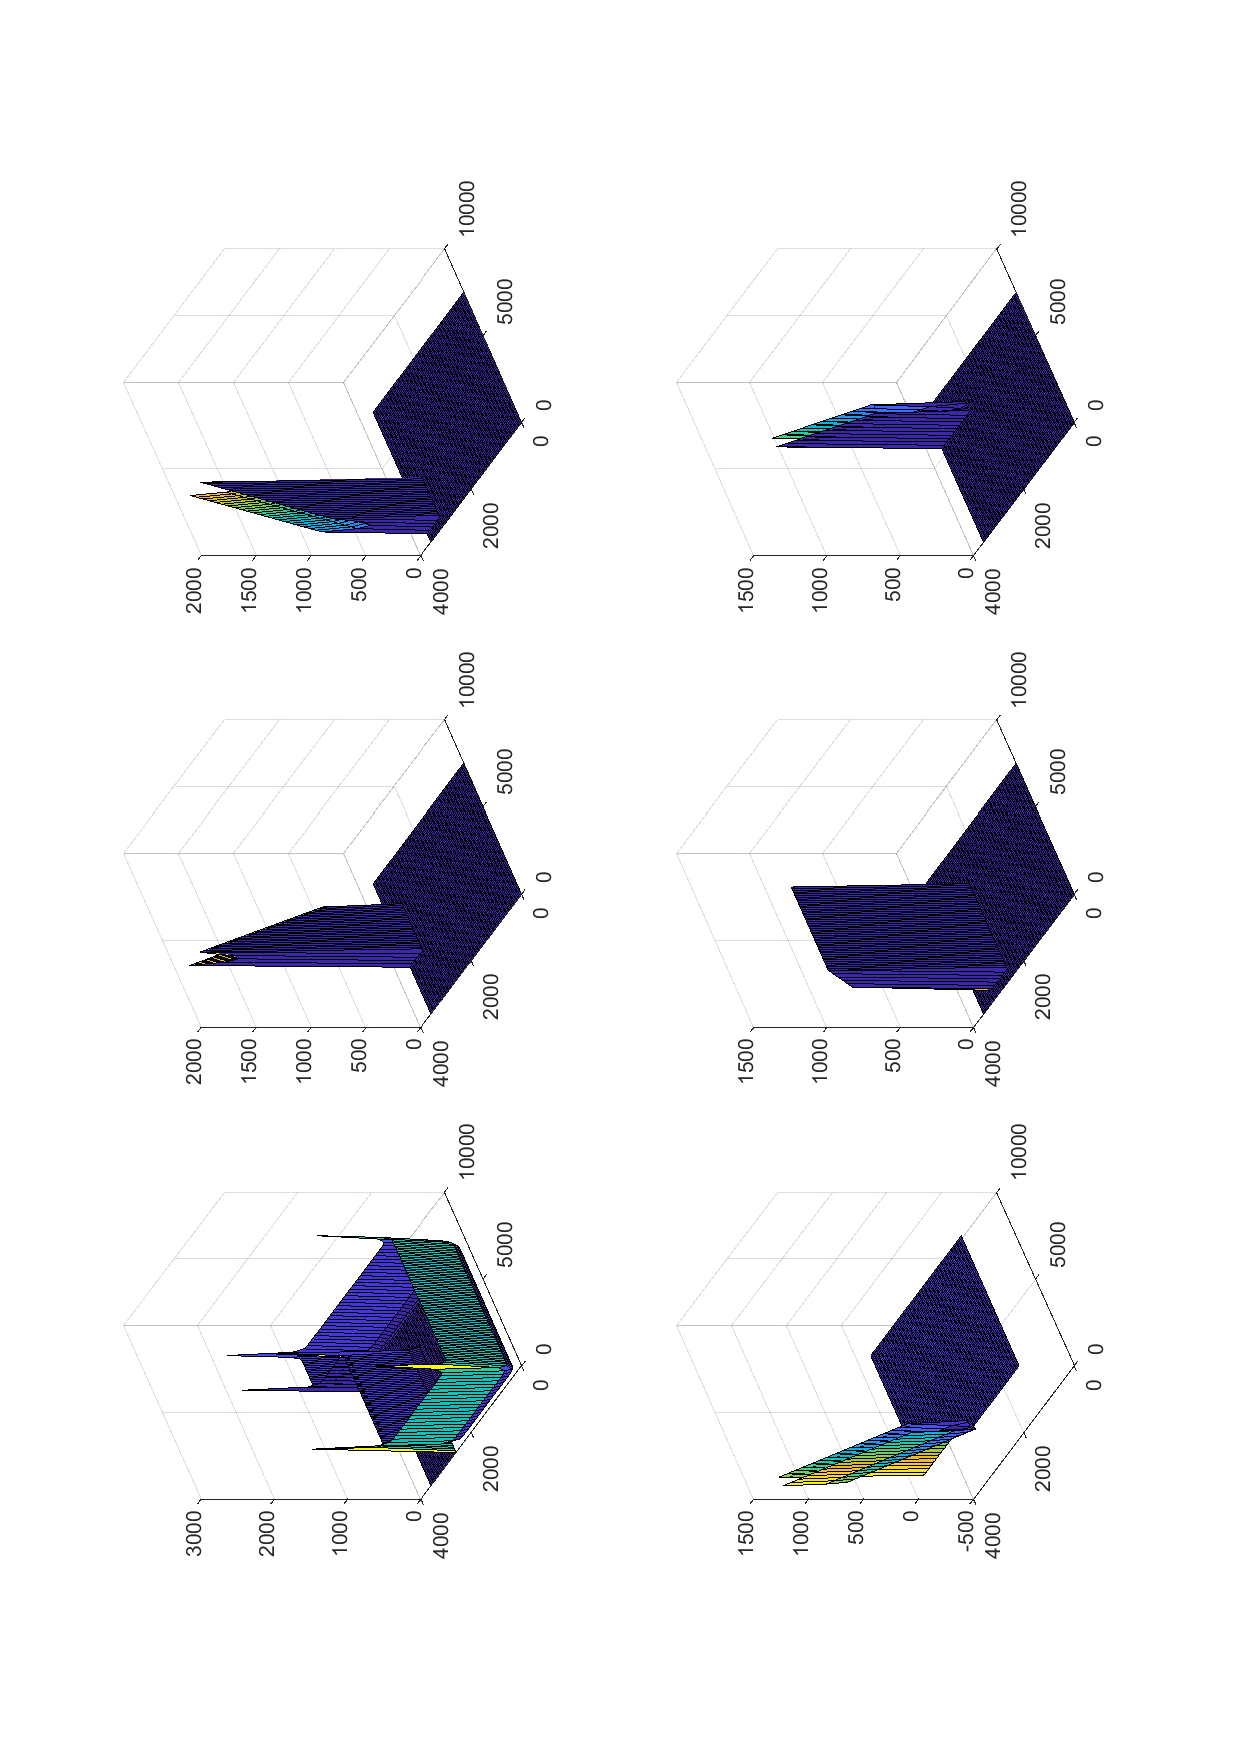
\includegraphics[width=0.8\textwidth,angle=-90]{grafiken/EinzelZonen.pdf}
	\caption{Potentialfeld der einzel Zonen}
	\label{fig:Poteinzeln}
\end{figure}

\begin{figure}
	\centering	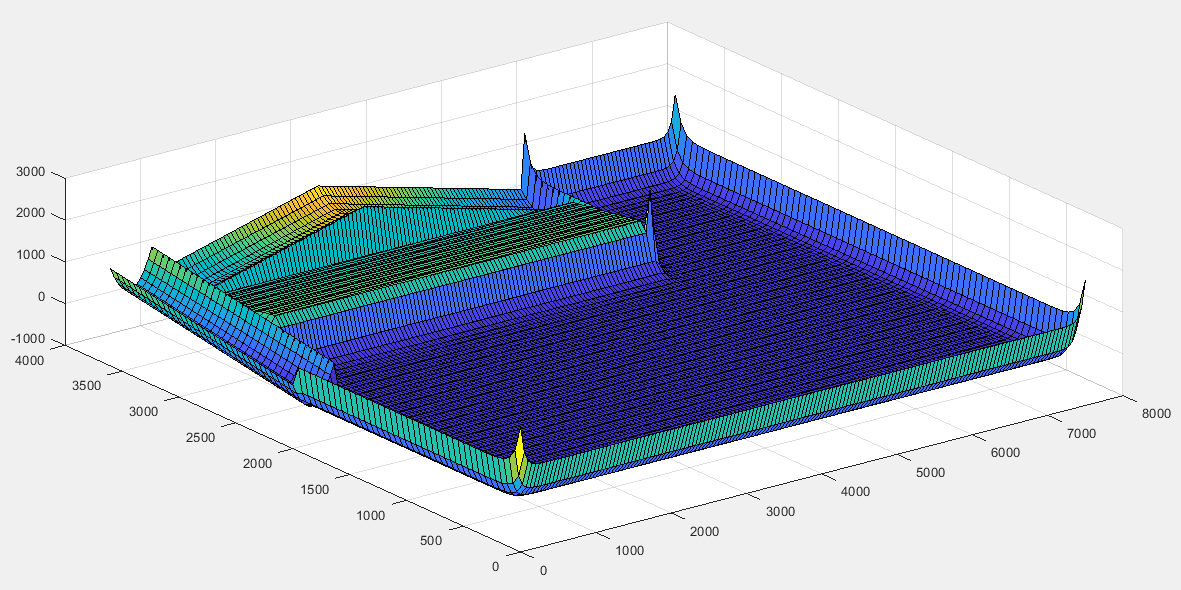
\includegraphics[width=0.8\textwidth]{grafiken/Potentialfeld_ohne_2schraege.png}
	\caption{Potentialfeld der Roboter Umwelt ohne Rausf�hrung}
	\label{fig:PotUmweltohne}
\end{figure}

\begin{figure}
	\centering	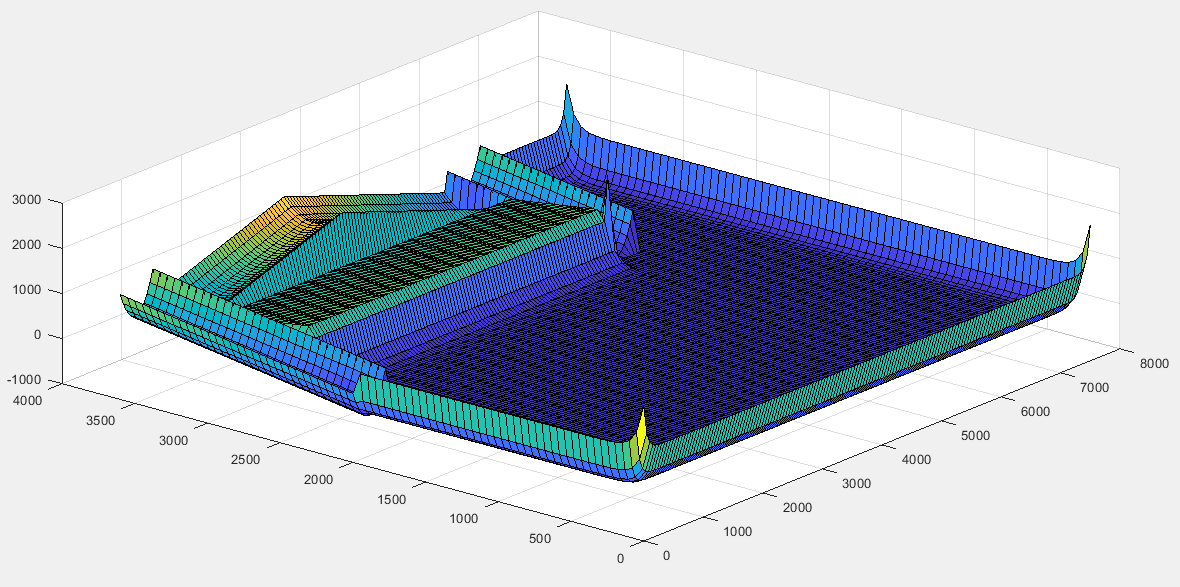
\includegraphics[width=0.8\textwidth]{grafiken/Potentialfeld_mit_2schraegen.png}
	\caption{Potentialfeld der Roboter Umwelt mit Rausf�hrung}
	\label{fig:PotUmweltmit}
\end{figure}

\subsection{Robotino,Stationen und IR-Hindernisse}\label{sec:PotRob}
Die Robotinos, die Stationen und die IR-Hindernisse werden im Potentialfeld als gau�sche radiale Basisfunktion betrachtet. Die genutzte Funktion ist unter \eqref{fun:H_gaus} definiert. Da sich die gau�sche radiale Basisfunktion aufgrund der genutzten e-Funktion gut ableiten l�sst, wird diese Funktion genutzt, um ein absto�endes Potential zu generieren. Das Potentialfeld der gau�schen radialen Basisfunktion ist in Abbildung \ref{fig:PotRobotino} dargestellt. Dabei wird f�r die Stationen eine konstante Position eingestellt. Die Position des Robotinos und der IR-Hindernisse werden als flexibel betrachtet, da sie w�hrend der Laufzeit bestimmt werden m�ssen.

\begin{align}
\label{fun:H_gaus}
H_{Hindernis}(x,y)=K\cdot e^{-\frac{(x-x_{pos})^2+(y-y_{pos})^2}{2\cdot \sigma^2}}
 \end{align}
 
\begin{figure}
	\centering	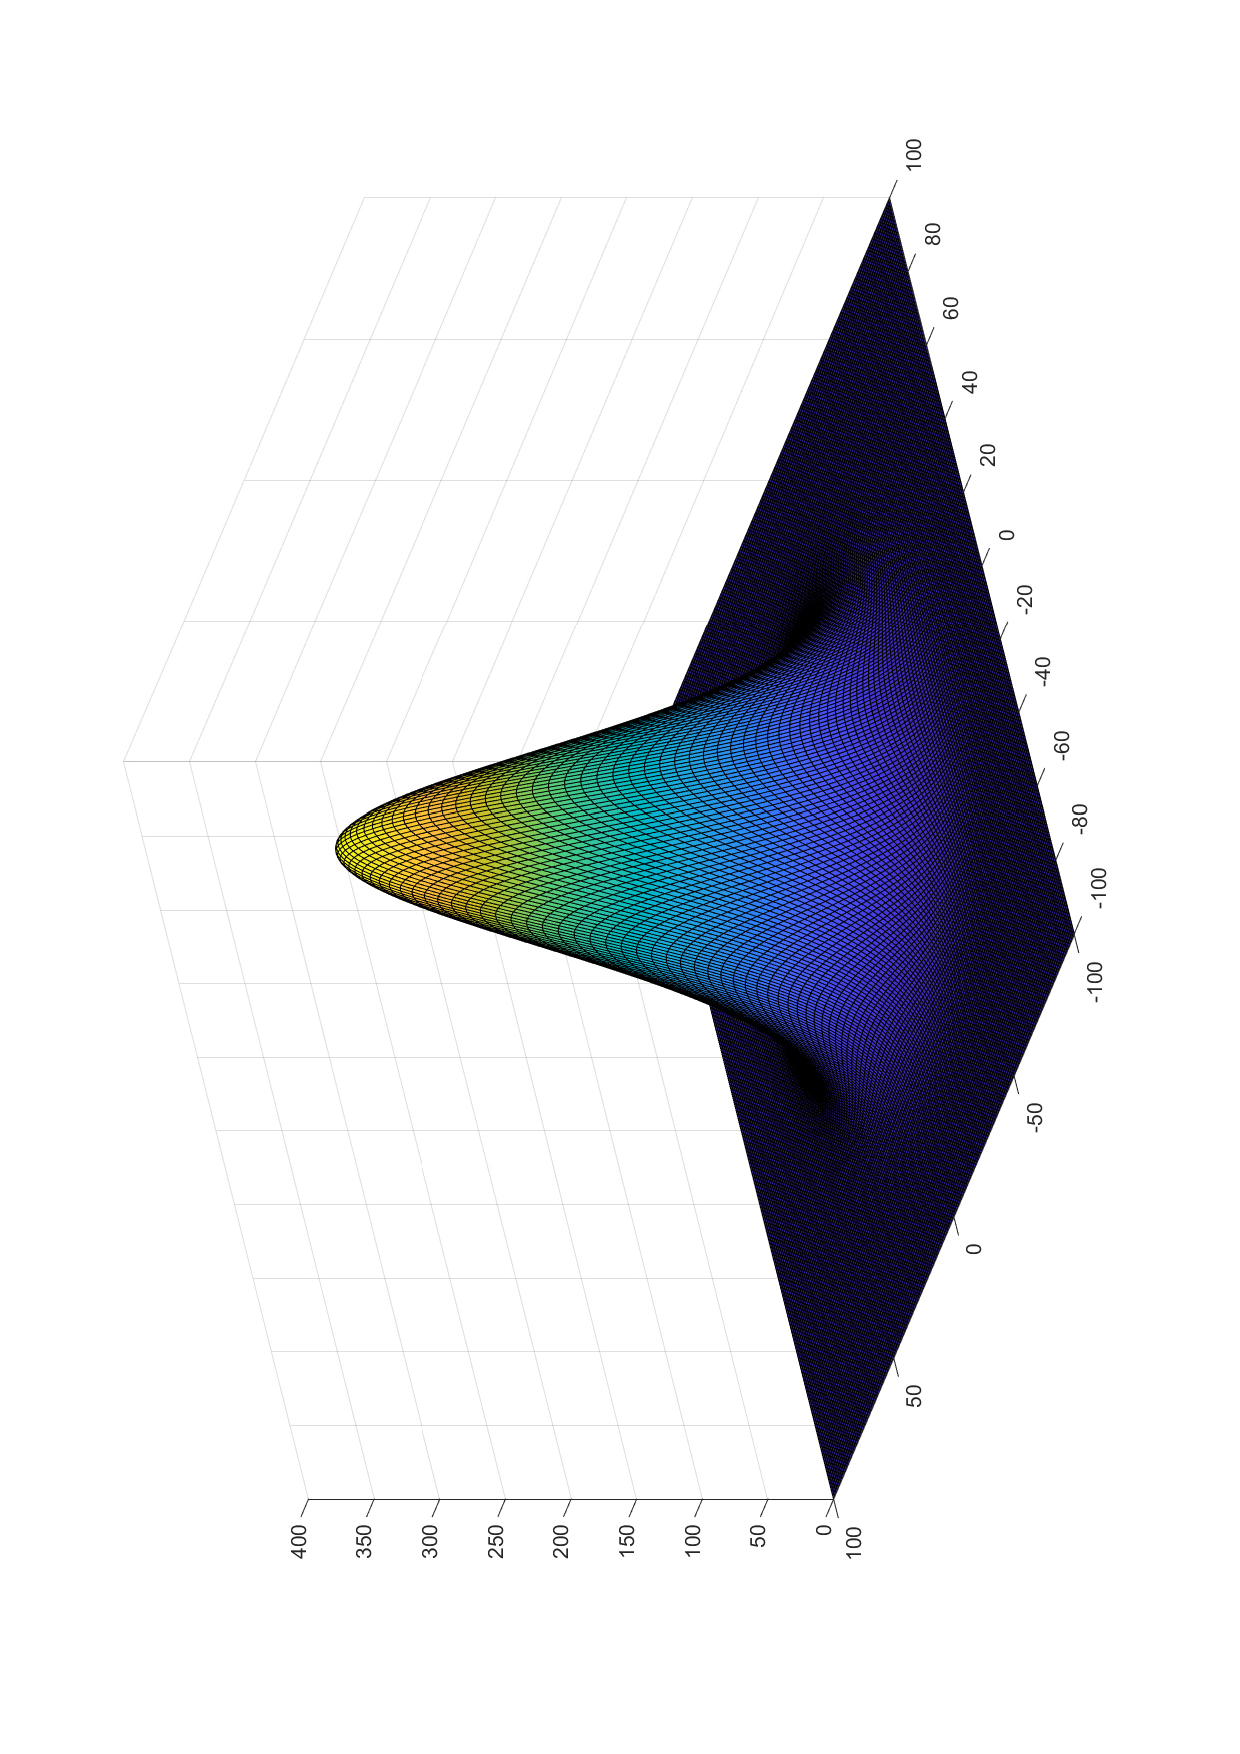
\includegraphics[width=0.8\textwidth,angle=-90]{grafiken/GaussKurve.pdf}
	\caption{Potentialfeld der gau�schen radialen Basisfunktion}
	\label{fig:PotRobotino}
\end{figure}

\subsection{Ziel} \label{sec:Ziel}
Das Ziel im Potentialfeld wird als Kegel mit konstantem Faktor realisiert. Dazu wird die in Gleichung \eqref{fun:H_Ziel} dargestellte Funktion genutzt. Um durch Tr�gheit verursachte Schwingungen um den Zielpunkt zu vermeiden, wird ein abstandsabh�ngiger Faktor als Filterung nachgeschaltet. Das Zielpotentialfeld ist in Abbildung \ref{fig:PotZiel} dargestellt.

\begin{align}
\label{fun:H_Ziel}
H_{Ziel}(x,y)= K \cdot \sqrt{(x-x_{Ziel})^2+(y-y_{Ziel})^2} 
 \end{align}
 
\begin{figure}
	\centering	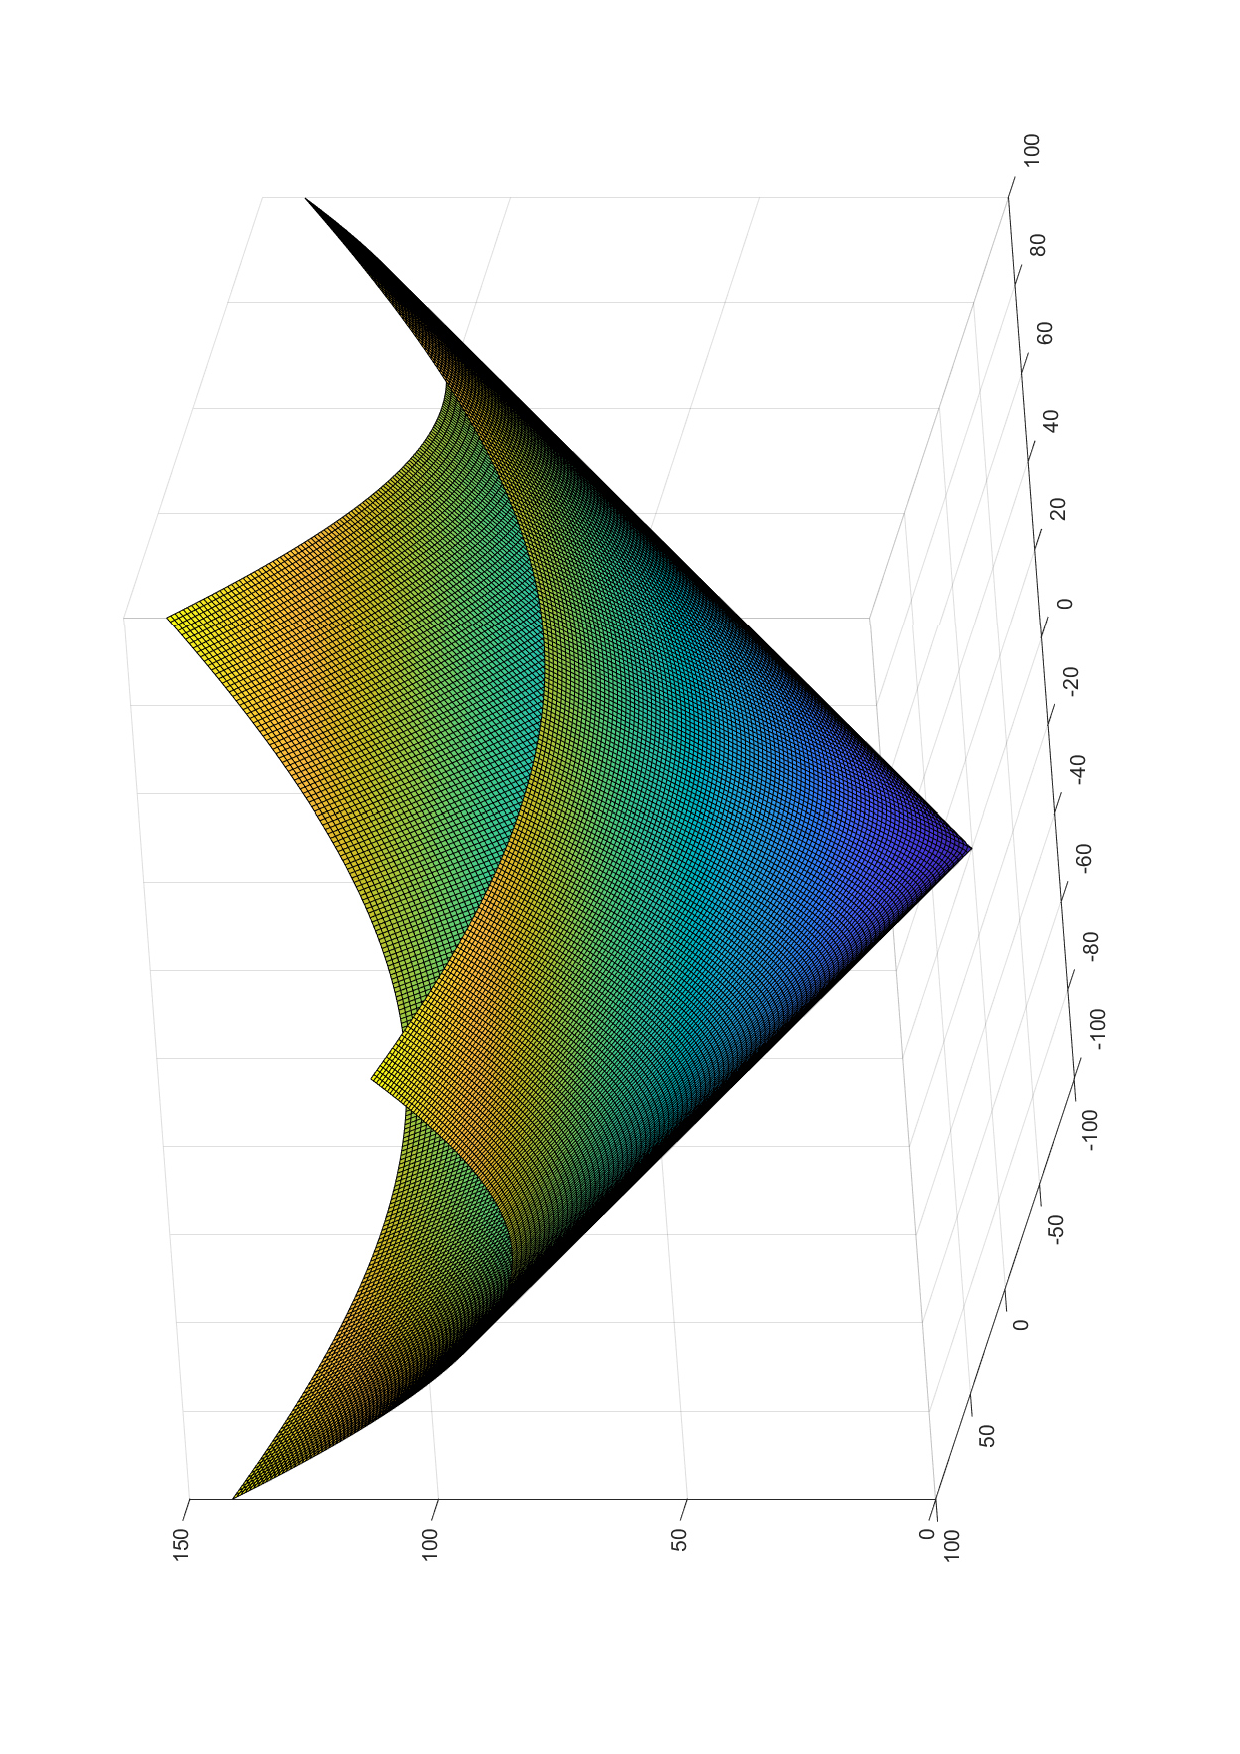
\includegraphics[width=0.8\textwidth,angle=-90]{grafiken/ZielKurve.pdf}
	\caption{Potentialfeld Ziel}
	\label{fig:PotZiel}
\end{figure}